Considera los dos triángulos que se muestran abajo en la Figura \ref{fig:20230323153911} (los triángulos no están dibujados a escala).

\begin{minipage}{0.6\textwidth}
    \textbf{¿Los dos triángulos son congruentes?}\\
    \emph{Escoge 1 respuesta:}\\
    \begin{choices}
        \choice Sí.
        \CorrectChoice No.
        \choice No hay suficiente información para decidir.
    \end{choices}
\end{minipage}%
\begin{minipage}{0.35\textwidth}
    \begin{figure}[H]
        \centering
        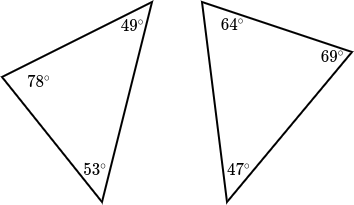
\includegraphics[width=\linewidth]{../images/20230323153911}
        \caption{}
        \label{fig:20230323153911}
    \end{figure}
\end{minipage}

\begin{solutionbox}{2.5cm}\footnotesize
    Dos triángulos son congruentes si tienen la misma forma y tamaño. En otras palabras, dos triángulos son congruentes si todos los lados y ángulos correspondientes son congruentes.

    En este caso, ya conocemos los tres ángulos en ambos triángulos y no hay dos que sean iguales.
    Por lo tanto, es imposible que los ángulos correspondientes sean congruentes y entonces los triángulos no son congruentes.

    \textbf{No, los triángulos no son congruentes.}
\end{solutionbox}